\subsubsection{Schema Codec}
\label{sec:Schema_Codec}

Die Wandlung des analogen Audio-Signale sowie die Rückwandlung der digitalen Signale vom Microcontroller  übernimmt ein TLV320AIC23B von Texas Instruments. Dieser Codec hat eine variable Sampling-Frequenz (8kHz-96kHz), einen Köpfhörer- und einen Mikrofon-Vorverstärker. Die Register des Codecs werden über I2C programmiert (wobei auch SPI möglich wäre), dazu wird der "Mode" Pin über eine Widerstand auf GND gezogen. Die gesampelten Daten wiederum werden über I2S an den Microcontroller übermittelt. Zusätzlich wird der 12.28 MHz Audio-Clock mit dem der Codec taktet von einem externen ECS-Quarz erzeugt (Abbildung \ref{fig:Schema_Codec}). 

\begin{figure} [H]
\begin{center}
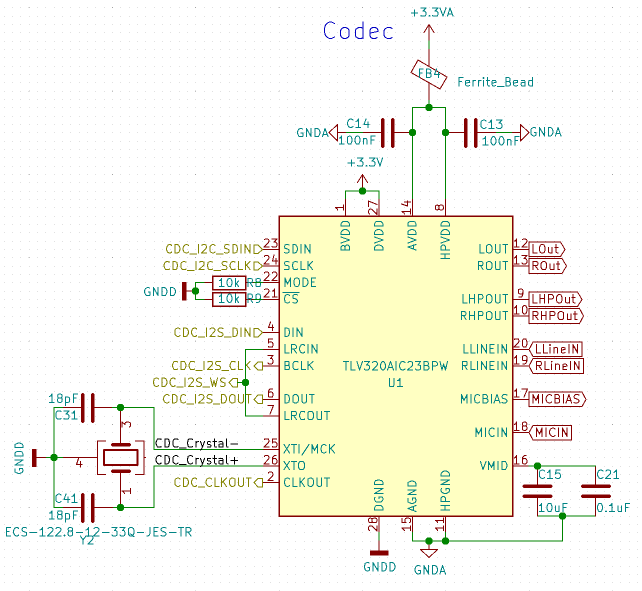
\includegraphics[scale=0.5]{../graphics/Schema_Codec.png}
\caption{TLV320AIC23B Codec von Texas Instruments}
\label{fig:Schema_Codec}
\end{center}
\end{figure}

Die Analog-Speisung des TLVs wird neben den 100nF Stütz-Kondensatoren zusätzlich von einem Ferrit Bead geglättet. Damit wird sichergestellt, dass keine ungewollten hochfrequente Spitzen in der Speisung das Audio-Signal verfälschen.

In den nachfolgenden Unterkapiteln wird genauer auf die In- und Outputs des DSP-Boards, beziehungsweise deren äusseren Beschaltung eingegangen.


\paragraph{Line Input}
\label{par:LineIN}

\begin{figure} [H]
\begin{center}
 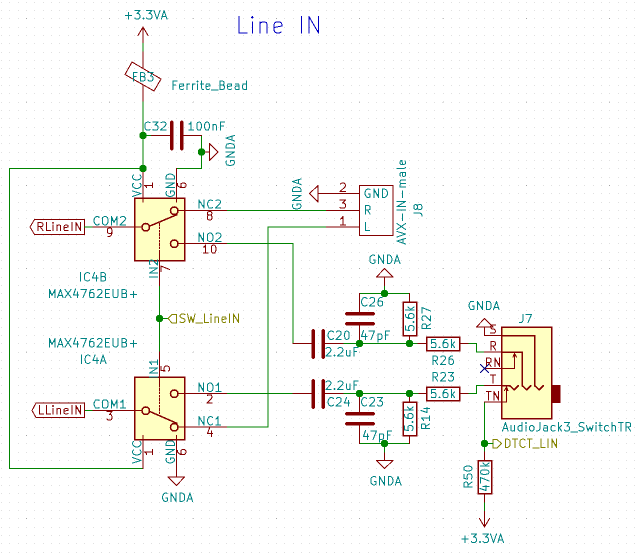
\includegraphics[scale=0.5]{../graphics/Schema_LineIN.png}
\caption{}
\label{fig:Schema_LineIN}
\end{center}
\end{figure}

\paragraph{Line Output}
\label{par:LineOUT}

\begin{figure} [H]
\begin{center}
 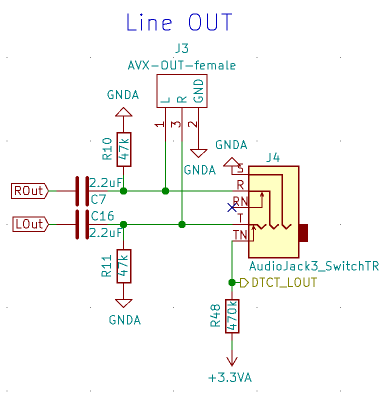
\includegraphics[scale=0.5]{../graphics/Schema_LineOUT.png}
\caption{}
\label{fig:Schema_LineOUT}
\end{center}
\end{figure}


\paragraph{Headphone Output}
\label{par:HPOUT}


\begin{figure} [H]
\begin{center}
 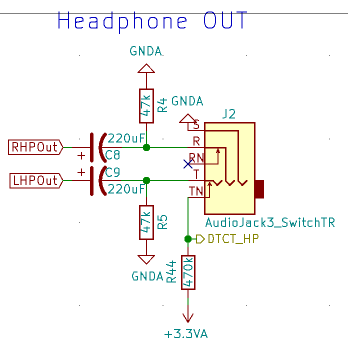
\includegraphics[scale=0.5]{../graphics/Schema_HPOUT.png}\caption{}
\label{fig:Schema_HPOUT}
\end{center}
\end{figure}




\paragraph{Mikrofon Input}
\label{par:MicIN}

\begin{figure} [H]
\begin{center}
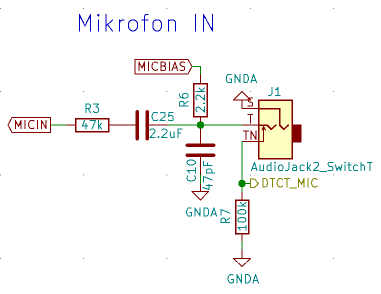
\includegraphics[scale=0.5]{../graphics/Schema_MicIN.png}
\caption{}
\label{fig:Schema_MicIN}
\end{center}
\end{figure}

\begin{figure} [H]
\begin{center}
 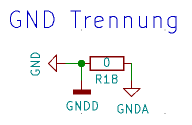
\includegraphics[scale=0.5]{../graphics/Schema_GND.png} 
\caption{}
\label{fig:Schema_GND}
\end{center}
\end{figure}



 